\begin{frame}{\insertsubsection}

  \begin{columns}
    \begin{column}{.6\textwidth}
      \begin{itemize}
      \item<1-> Rust Working Groups
        \begin{itemize}
        \item Networking services
        \item WebAssembly
        \item CLI Apss
        \item Embedded Devices
        \item Lang and compiler working groups (WG-NLL, WG-UCG, WG-Traits and
          etc)
        \end{itemize}
      \item<2-> This week in Rust (This week in \texttt{ProjectName})
      \item<3-> Meetups
      \item<4-> Chats (IRC, Telegram, Gitter, Matrix, Jabber)
      \item<5-> Blogs (\href{https://blog.rust-lang.org/}{Official},
        \href{https://readrust.net/}{Read Rust}, Core Developers, many others)
      \end{itemize}
    \end{column}
    \begin{column}{.4\textwidth}
      \center%
      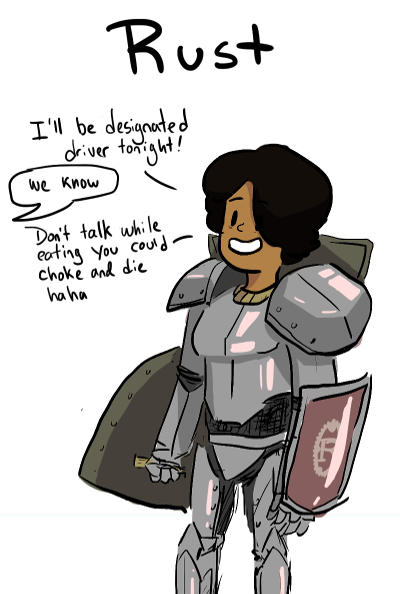
\includegraphics[height = .8\textheight]{rust_knight.png}
    \end{column}
  \end{columns}

  \note<1>{

    Кроме того, что Rust --- open source разработка, как я уже говорил, и все
    фичи обсуждаются и принимаются всеми, \textbf{существуют рабочие группы}.
    Каждая группа отвечает за свою область, вступить в них можно, если активно
    проявляешь себя в той или иной области. Каждая группа отчитывается за
    проделанную работу, а также составляет планы на будущее.

  }

  \note<2>{

    \textbf{Каждую неделю постятся новости}, полезные ссылки, статьи, цитаты,
    информация о сходках, о том, какие \textbf{изменения в компиляторе}
    разработали, какие \textbf{RFC} принимаются, что стабилизируется,
    \textbf{работа}, \textbf{проекты, которым нужна помощь} и о прочем.
    \textbf{Не требуется собирать свежую информацию} по крупицам со всего
    интернета.

    Кроме этого по некоторым проектам также каждую неделю постится информация.

  }

  \note<3>{

    По Rust очень много сходок по всему миру. Кроме того, что за год проходит по
    \textbf{две официальные конференции}, во всех странах мирах создаются
    небольшие сходки. \textbf{В Питере} тоже есть такая, собираемся \textbf{в
      JetBrains примерно 2 раза месяц}. В Москве --- \textbf{организатор
      Kaspersky}.

  }

  \note<4>{

    В чатах создано множество тематических групп. В том числе русскоязычных: и
    по Web разработке, и по embedded, и просто по Rust.

  }

  \note<5>{

    По Rust очень \textbf{много информации в блогах}. Есть много
    структурированной информации \textbf{на официальных сайтах}, есть
    \textbf{блоги core разработчиков} и множество других. \textbf{Core
      разработчики устраивают офисные часы} --- раз в 2 недели задаются
    животрепещущий вопрос, разработчик чётко с примерами отвечает.

    \textbf{Rust сообщество очень дружелюбное!} По вопросам в остальных языках
    могут и заклевать.

  }

\end{frame}
